%
% Poster latex file for ADASS 2018
% Pey Lian Lim (lim@stsci.edu)
% Eric R. Jeschke (eric@naoj.org)
%
% [top-level file]
\nonstopmode

\documentclass[]{article}
\usepackage{graphicx}
% where can I find the graphics that will be imported for this version
\graphicspath{{./figures/}}

% Using \fbox you can draw a nice razor-thin border around images
\setlength\fboxsep{0pt}
\setlength\fboxrule{0.5pt}

% in case you want to embed any hyperlinks
%\usepackage{hyperref}

% for + and - signs in setting width etc
\usepackage{calc}

% scalable fonts
\usepackage[quiet]{fontspec}
\setmainfont[Mapping=tex-text,Scale=2.1]{DejaVu Serif}
\setsansfont[Mapping=tex-text,Scale=2.1]{DejaVu Sans}
\setmonofont[Mapping=tex-text,Scale=2.1]{DejaVu Sans Mono}
%\setmainfont[Mapping=tex-text,Scale=1.0]{Times New Roman}
%setsansfont[Mapping=tex-text,Scale=1.0]{Arial}
%setmonofont[Mapping=tex-text,Scale=1.0]{Courier New}

% for multiple columns
\usepackage{multicol}

% fancy boxes
\usepackage{fancybox}

% uncomment the actual desired size
%\def\mypaperwidth{33.11in} \def\mypaperheight{46.81in}    % A0
\def\mypaperwidth{27.83in} \def\mypaperheight{39.37in}     % B1
%\def\mypaperwidth{23.39in} \def\mypaperheight{33.1124in}  % A1
%\def\mypaperwidth{8.27in} \def\mypaperheight{11.69in}  % A4
\def\imgwd{6.0in}  % define image widths
% margin around edge of page
\def\mymargin{1in}

%% \def\mypaperwidth{11in} \def\mypaperheight{17.0in}     % Tabloid
%% \def\imgwd{2.5in}  % define image widths
%% \def\mymargin{0.25in}

% painful TeX calculation of 2*margin
\dimen87=\mymargin
\multiply\dimen87 by 2
\def\mydblmargin{\dimen87}

\usepackage[paperwidth=\mypaperwidth, paperheight=\mypaperheight,
            % margins are calculated from the trim + no print area
            top=\mymargin, bottom=\mymargin,
            left=\mymargin, right=\mymargin]{geometry}

\begin{document}

% dimensions of main writing area of page
\setlength{\textwidth}{\mypaperwidth-\mydblmargin}
%\setlength{\textwidth}{13in}
\setlength{\textheight}{\mypaperheight-\mydblmargin}

% TeX defines the content to begin at 1in offset from the side and
% top of the document (seemingly somewhat independent of margin
% settings).  These specify offsets to be added to the 1in defaults.
% You can calculate these or just tweak them until you get the result
% that you like.
\setlength{\hoffset}{-1.0in}
\setlength{\voffset}{-1.0in}

% width of margin notes area
\setlength{\marginparwidth}{0in}
% distance between margin and paragraph
\setlength{\marginparsep}{0in}

% footer configuration
\setlength{\footskip}{1em}

% header configuration
\setlength\headheight{0in}
\setlength\headsep{1em}

% margin tweaking
\setlength{\topmargin}{0.0in}
\setlength{\oddsidemargin}{1in}
% LEFT margin on even pages
\setlength{\evensidemargin}{1in}

% define explicitly set paragraph spacing
\newcommand{\para}{\vspace*{1em}}

\title{{\tt stginga}: Ginga Plugins for Data Analysis and Quality Assurance of
            HST and JWST Science Data}
\author{P. L. Lim (STScI) and E. R. Jeschke (NAOJ)}

% paragraph indentations
\setlength{\parindent}{0in}
% amount of space before each new paragraph begins
\setlength{\parskip}{0pt}

% comment to force even justification
\raggedright

%\begin{document}

\pagestyle{empty}

% interior facing page for book version
\begin{minipage}[t]{0.8\linewidth}
  \vspace{0pt}
\begin{center}
{\huge {\tt stginga}: Ginga Plugins for Data Analysis and Quality Assurance of
            HST and JWST Science Data }\\

\vspace*{1.5em}
Pey Lian Lim ({\tt lim@stsci.edu}),
Space Telescope Science Institute \\
Eric R. Jeschke ({\tt eric@naoj.org}),
National Astronomical Observatory of Japan
\end{center}
\end{minipage}
\hfill
\begin{minipage}[t]{0.15\linewidth}
  \vspace{0pt}
  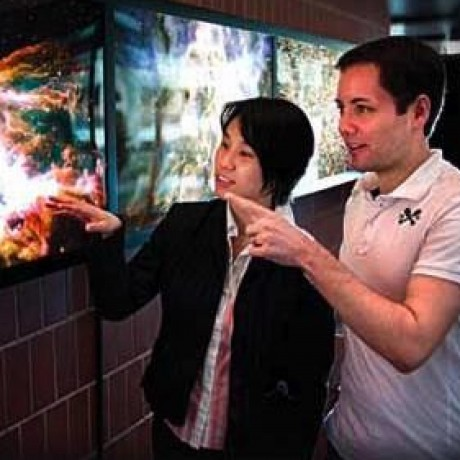
\includegraphics[width=2in]{pllim} \\
  {P. L. Lim}
\end{minipage}
%\vspace*{0in}
\vspace*{2em}

\noindent\hrulefill

\raggedcolumns
\setlength{\columnseprule}{1pt}
\setlength{\columnsep}{2em}

\medskip
\begin{multicols}{3}

\section*{Abstract}
{\tt stginga}\cite{stginga} is an image visualization package to assist
in data analysis and quality assurance of science data from Hubble Space
Telescope (HST) and James Webb Space Telescope (JWST).  It is based on the
Ginga\cite{ginga} toolkit for building scientific viewers.
In this poster, we will describe the main plugins developed for data
analysis and quality assurance tasks with {\tt stginga}.  We also discuss the
basic outline of writing a Ginga plugin, with pointers to documentation
and examples.

\section*{Introduction}

\begin{center}
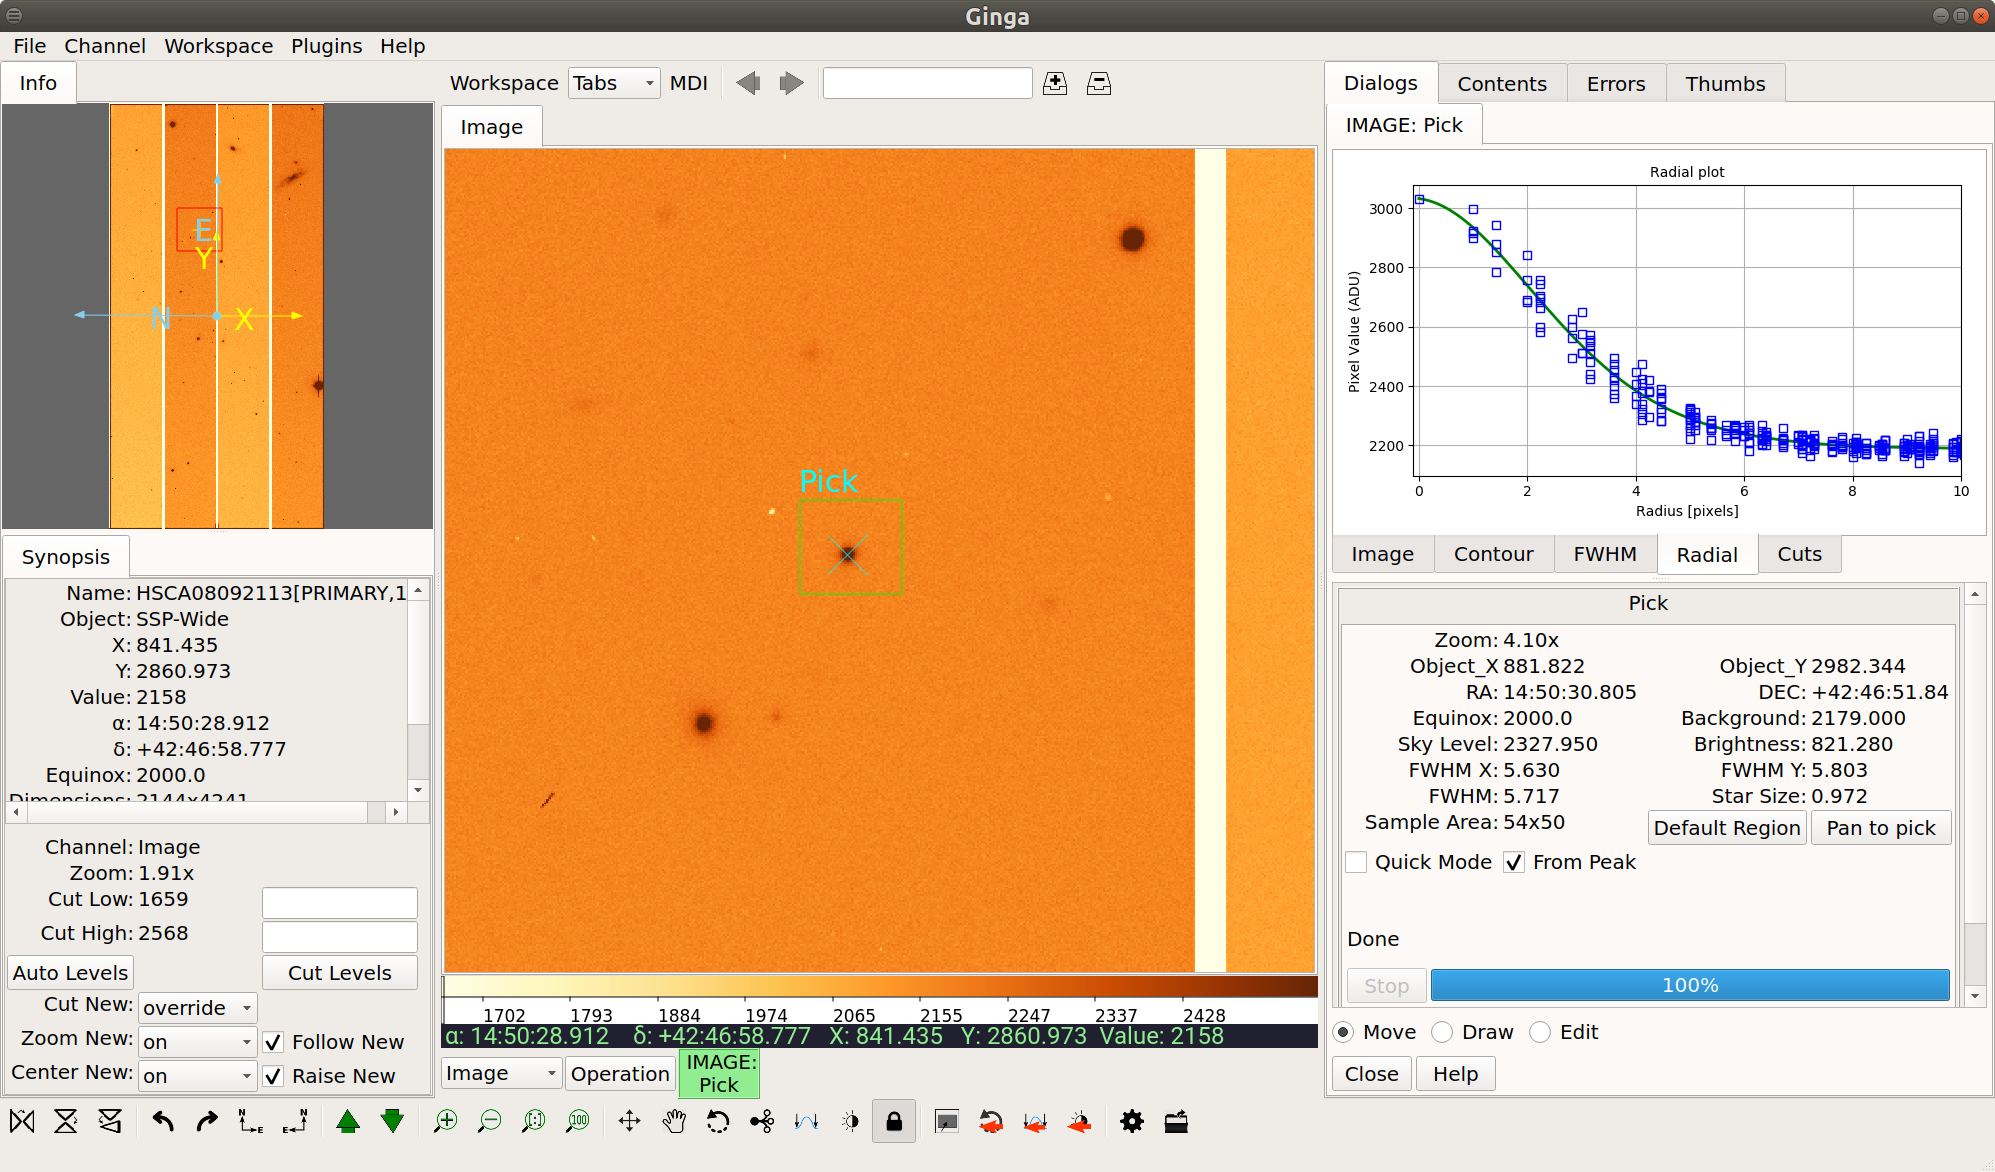
\includegraphics[width=8in]{ref_viewer}
\label{fig:refviewer}
\vspace*{0.4em}
{\small\em Figure 1: The Ginga reference viewer.}
\end{center}

\para
Ginga\cite{Jeschke15A} is a Python package that
implements a toolkit for building scientific viewers.  It provides
a \emph{reference viewer} (see Fig. 1), which features
a plugin architecture in which nearly every graphical feature of the
program is implemented by a Python plugin.
By implementing some new plugins for the HST and JWST data analysis and
quality assurance tasks, and combining these with a curated selection of
the distributed ``stock'' plugins, we were able to fairly quickly
develop a tool for use in the HST and JWST community.

\para
Ginga plugins are separated into global and local ones. A global plugin applies
to all images across all channels; thus, only once instance can be opened
in the whole Ginga session.
Meanwhile, a local plugin is associated with the channel it is started from;
therefore, one instance can be opened per channel and different instances
can be configured separately in the same Ginga session.
Plugins are currently not available when Ginga is used as part of Jupyter
Notebook/Lab. However, they are usable in a limited way via Ginga's remote
control (RC) interface, which will not be covered here.

\para
Currently, all the plugins are available in {\tt stginga} are local plugins.
Some plugins currently in Ginga originated from {\tt stginga}
(e.g., {\em ChangeHistory}, {\em SaveImage}, {\em TVMark}, and {\em TVMask})
when they were identified to be useful in general beyond HST or JWST.
All the screenshots shown in this poster used Qt5 backend, although they should
also work in Qt4, GTK 2, and GTK 3.

\section*{BackgroundSub}

\para
\begin{center}
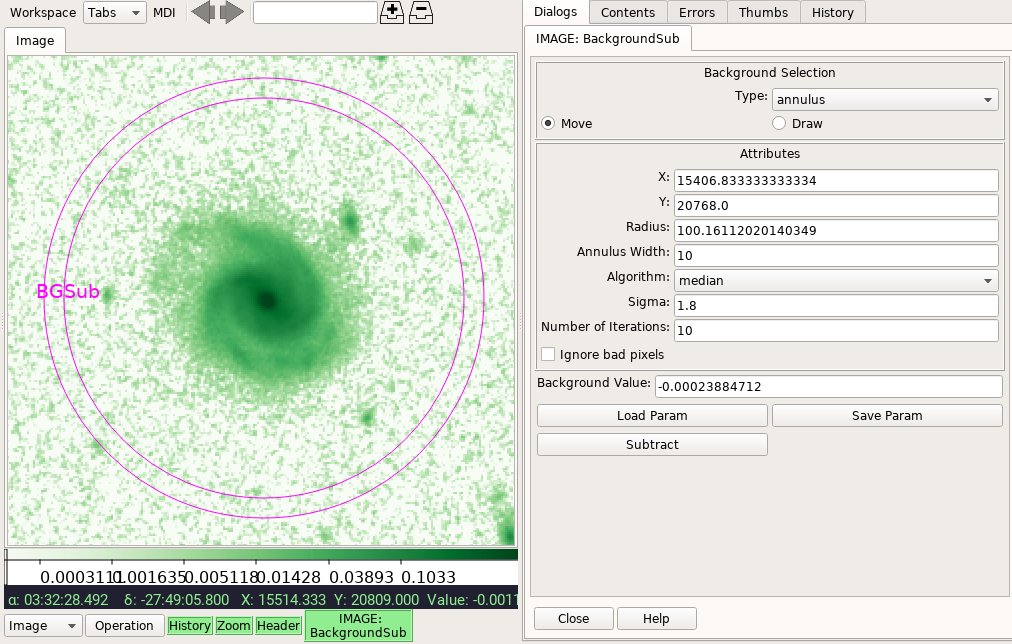
\includegraphics[width=8in]{plugin_backgroundsub} \\
\vspace*{0.4em}
\label{fig:plugin_backgroundsub}
{\small\em Figure 2: BackgroundSub plugin for background subtraction.}
\end{center}

\para
Something about the plugin.

\section*{BadPixCorr}

\para
\begin{center}
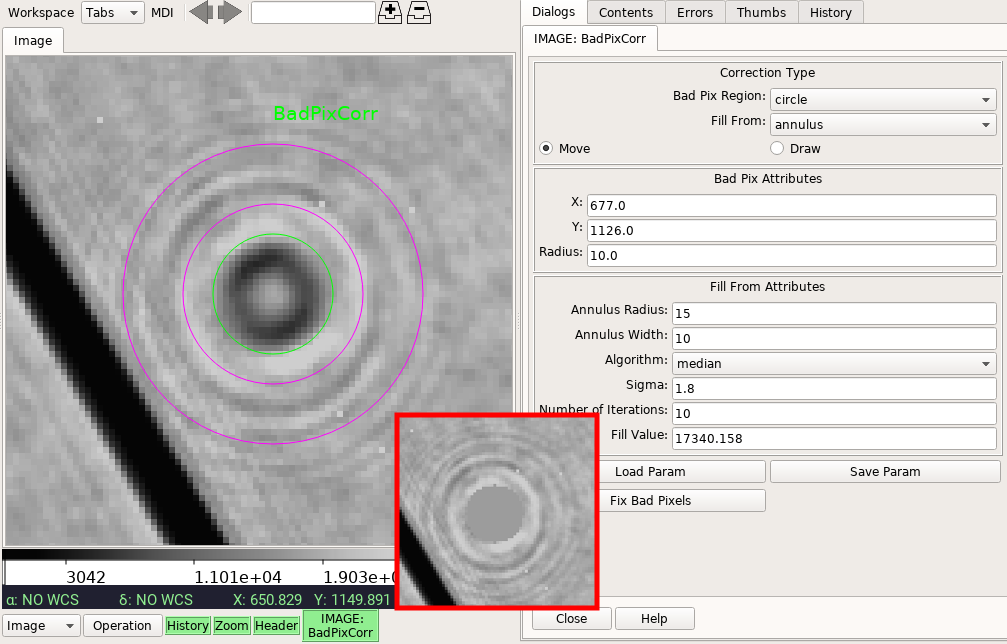
\includegraphics[width=8in]{plugin_badpixcorr.png}
\label{fig:plugin_badpixcorr}
\vspace*{0.4em}
{\small\em Figure 3: BadPixCorr plugin for bad pixel correction.}
\end{center}

\para
Something.

\para
Something something.

\section*{DQInspect}

\para
\begin{center}
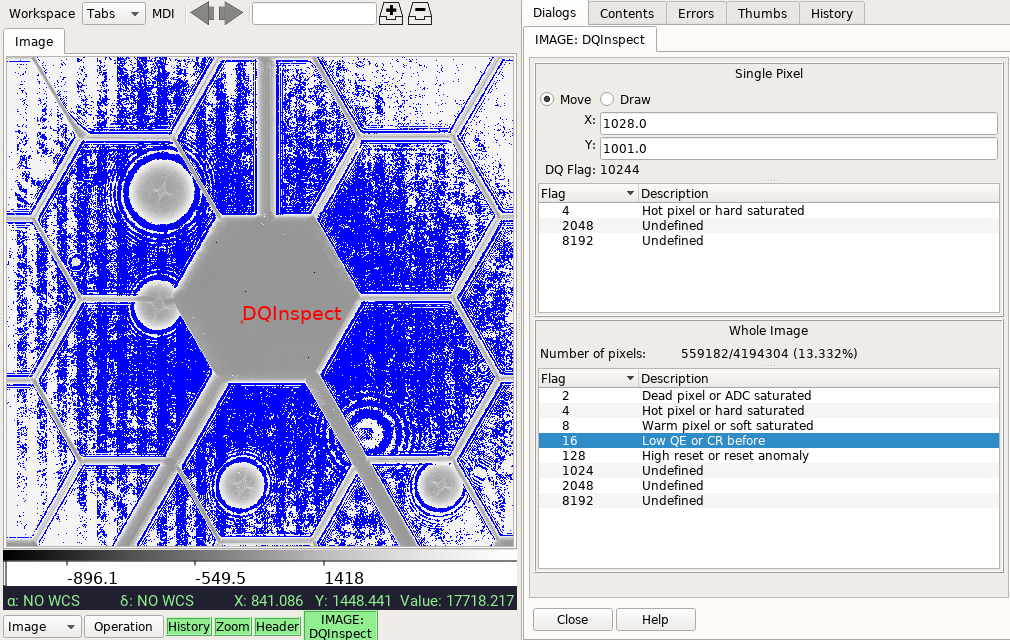
\includegraphics[width=8in]{plugin_dqinspect} \\
\vspace*{0.4em}
\label{fig:plugin_dqinspect}
{\small\em Figure 4: DQInspect plugin for data quality inspection.}
\end{center}

\para
Something something.

\section*{SNRCalc}

\para
\begin{center}
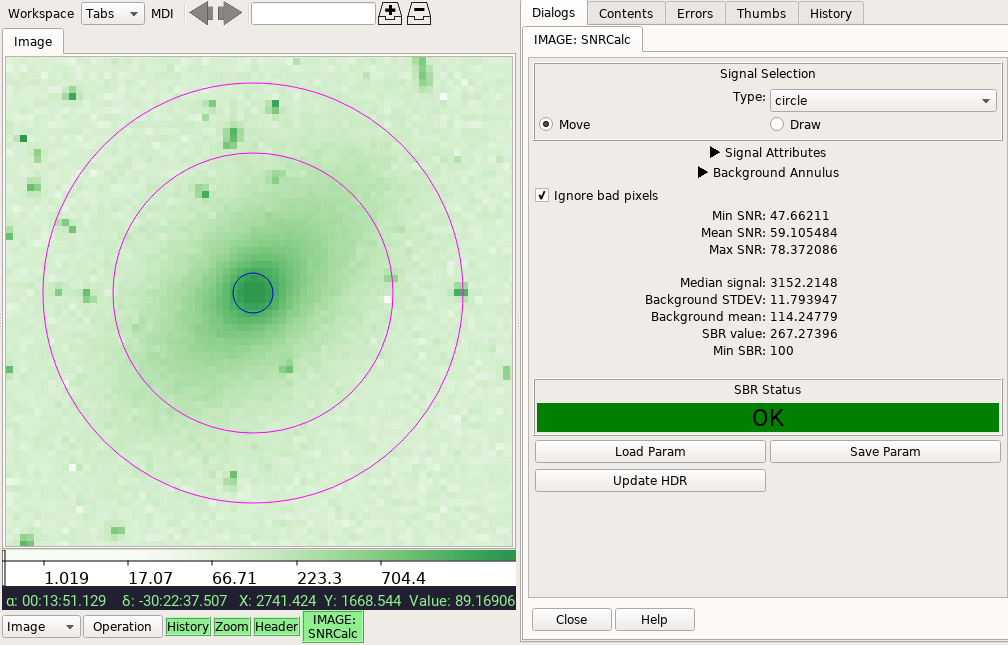
\includegraphics[width=8in]{plugin_snrcalc} \\
\vspace*{0.4em}
\label{fig:plugin_snrcalc}
{\small\em Figure 5: SNRCalc plugin for SNR calculation.}
\end{center}

\para
Something something.

\section*{Writing a Ginga plugin}

\para
Something. Maybe code snippet for the template.

\para
Something.

\section*{Conclusion}

{\tt stginga} utilizes Ginga plugins to support HST and JWST data analysis,
which includes background subtraction, bad pixel correction, data quality flags
inspection, and signal-to-noise calculations.

\para
Writing Ginga plugins can be an expedient way to develop graphical data
analysis and quality assurance tasks, by leveraging the combination of
Python, a lean Ginga plugin API, and the burgeoning number of open-source
astronomical Python modules.

\para
Both {\tt stginga} and {\tt ginga} are installable via {\tt pip}. Alternately,
if you use {\tt conda}, they are also available on AstroConda\cite{astroconda},
in addition to {\tt ginga} being in  {\tt conda-forge} too. Their development
versions could be cloned from GitHub. Both are open-source and licensed under
3-clause BSD.

\bibliographystyle{abbrv}
\bibliography{poster}

\end{multicols}

\end{document}
